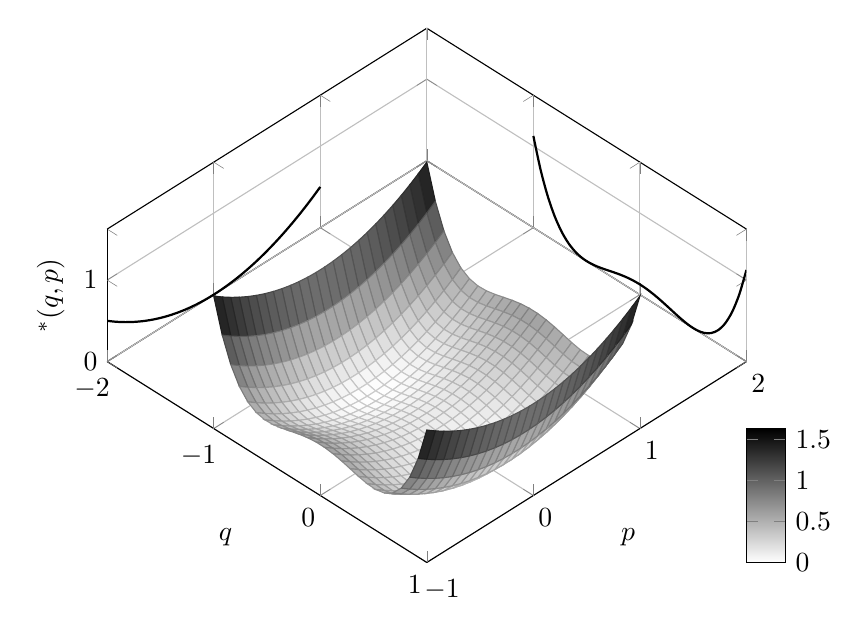
\begin{tikzpicture}[
  declare function = {lambda=2;},
  declare function = {mu=1;},
  declare function = {kin=(x^2)/2;},
  declare function = {pot(\l,\m)=\l*x^4 - \m*x^2 + (\m^2)/(4*\l);},
  declare function = {H(\l,\m)=\l*x^4 - \m*x^2  + (\m^2)/(4*\l)+ (y^2)/2;}]
  \begin{axis}[
    colormap  = {whiteblack}{color(0cm)  = (white);color(1cm) = (black)},
    width          = 0.8\linewidth,
    view           = {45}{65},
    enlargelimits  = false,
    grid           = major,
    domain         = -1:1,
    y domain       = -1:1,
    samples        = 26,
    xlabel         = $q$,
    ylabel         = $p$,
    zlabel         = {$\Ha^*(q,p)$},
    colorbar,
    colorbar style = {
      at     = {(1,0)},
      anchor = south west,
      height = 0.25*\pgfkeysvalueof{/pgfplots/parent axis height},
     % title  = {$P(x_1,x_2)$}
    }
  ]
    \addplot3 [surf] {H(lambda,mu)};
    \addplot3 [domain=-1:1,samples=31, samples y=0, thick, smooth]
     (x,2,{pot(lambda,mu)});
    \addplot3 [domain=-1:1,samples=31, samples y=0, thick, smooth]
      (-2,x,{kin});

    %\draw [black!50] (axis cs:-1,0,0) -- (axis cs:4,0,0);
    %\draw [black!50] (axis cs:0,-1,0) -- (axis cs:0,4,0);

    %\node at (axis cs:-1,1,0.18) [pin=165:$P(x_1)$] {};
    %\node at (axis cs:1.5,4,0.32) [pin=-15:$P(x_2)$] {};
  \end{axis}
\end{tikzpicture}